
\documentclass[border=8pt, multi, tikz]{standalone} 
\usepackage{import}
\subimport{../layers/}{init}
\usetikzlibrary{positioning}
\usetikzlibrary{3d} %for including external image 

\def\ConvColor{rgb:yellow,5;red,2.5;white,5}
\def\DcnvColor{rgb:blue,5;green,2.5;white,5}
\def\ConvReluColor{rgb:yellow,5;red,5;white,5}
\def\PoolColor{rgb:red,1;black,0.3}
\def\ReluColor{rgb:red,2;blue,0.1}
\def\UnpoolColor{rgb:blue,2;green,1;black,0.3}
\def\FcColor{rgb:blue,5;red,2.5;white,5}
\def\FcReluColor{rgb:blue,5;red,5;white,4}
\def\SoftmaxColor{rgb:magenta,5;black,7}   
\def\SumColor{rgb:blue,5;green,15}

\newcommand{\copymidarrow}{\tikz \draw[-Stealth,line width=0.8mm,draw={rgb:blue,4;red,1;green,1;black,3}] (-0.3,0) -- ++(0.3,0);}

\begin{document}
\begin{tikzpicture}
\tikzstyle{connection}=[ultra thick,every node/.style={sloped,allow upside down},draw=\edgecolor,opacity=0.7]
\tikzstyle{copyconnection}=[ultra thick,every node/.style={sloped,allow upside down},draw={rgb:blue,4;red,1;green,1;black,3},opacity=0.7]

\node[canvas is zy plane at x=0] (temp) at (-2,0,0) {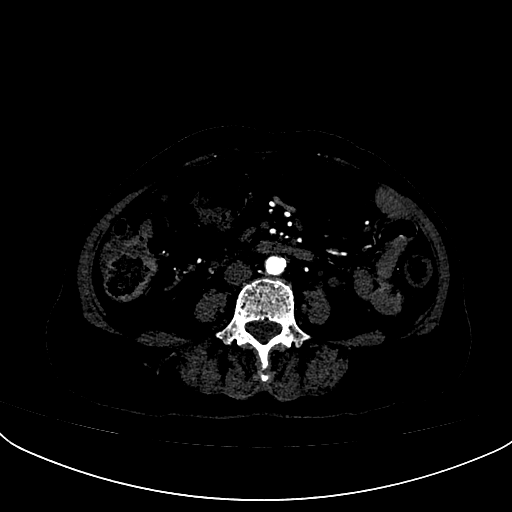
\includegraphics[width=8cm,height=8cm]{ id01_18_origin.png}};

\pic[shift={ (0,0,0) }] at (0,0,0) 
    {RightBandedBox={
        name=ccr_b1,
        caption=U-Net,
        xlabel={{ 64, 64 }},
        zlabel=256,
        fill=\ConvColor,
        bandfill=\ConvReluColor,
        height=35,
        width={ 2 , 2 },
        depth=35
        }
    };

\pic[shift={ (0,0,0) }] at (ccr_b1-east) 
    {Box={
        name=pool_b1,
        caption= ,
        fill=\PoolColor,
        opacity=0.5,
        height=28,
        width=1,
        depth=28
        }
    };

\pic[shift={(0.5,0,0)}] at (pool_b1-east) 
    {Box={
        name=conv1,
        caption=ResNet50,
        xlabel={{64, }},
        zlabel=256,
        fill=\DcnvColor,
        height=5,
        width=6,
        depth=5
        }
    };

\draw [connection]  (pool_b1-east)    -- node {\midarrow} (conv1-west);

\pic[shift={ (1,0,0) }] at (conv1-east) 
    {RightBandedBox={
        name=ccr_b2,
        caption= ,
        xlabel={{ 128, 128 }},
        zlabel=128,
        fill=\ConvColor,
        bandfill=\ConvReluColor,
        height=28,
        width={ 3.5 , 3.5 },
        depth=28
        }
    };

\pic[shift={ (0,0,0) }] at (ccr_b2-east) 
    {Box={
        name=pool_b2,
        caption= ,
        fill=\PoolColor,
        opacity=0.5,
        height=21,
        width=1,
        depth=21
        }
    };

\draw [connection]  (conv1-east)    -- node {\midarrow} (ccr_b2-west);

\pic[shift={(0.5,0,0)}] at (pool_b2-east) 
    {Box={
        name=conv2,
        caption=ResNet50,
        xlabel={{64, }},
        zlabel=256,
        fill=\DcnvColor,
        height=5,
        width=6,
        depth=5
        }
    };

\draw [connection]  (pool_b2-east)    -- node {\midarrow} (conv2-west);

\pic[shift={ (1,0,0) }] at (conv2-east) 
    {RightBandedBox={
        name=ccr_b3,
        caption= ,
        xlabel={{ 256, 256 }},
        zlabel=64,
        fill=\ConvColor,
        bandfill=\ConvReluColor,
        height=11,
        width={ 4.5 , 4.5 },
        depth=11
        }
    };

\pic[shift={ (0,0,0) }] at (ccr_b3-east) 
    {Box={
        name=pool_b3,
        caption= ,
        fill=\PoolColor,
        opacity=0.5,
        height=9,
        width=1,
        depth=9
        }
    };

\draw [connection]  (conv2-east)    -- node {\midarrow} (ccr_b3-west);

\pic[shift={(0.5,0,0)}] at (pool_b3-east) 
    {Box={
        name=conv3,
        caption=ResNet50,
        xlabel={{64, }},
        zlabel=256,
        fill=\DcnvColor,
        height=5,
        width=6,
        depth=5
        }
    };

\draw [connection]  (pool_b3-east)    -- node {\midarrow} (conv3-west);

\pic[shift={ (1,0,0) }] at (conv3-east) 
    {RightBandedBox={
        name=ccr_b4,
        caption= ,
        xlabel={{ 512, 512 }},
        zlabel=32,
        fill=\ConvColor,
        bandfill=\ConvReluColor,
        height=11,
        width={ 5.5 , 5.5 },
        depth=11
        }
    };

\pic[shift={ (0,0,0) }] at (ccr_b4-east) 
    {Box={
        name=pool_b4,
        caption= ,
        fill=\PoolColor,
        opacity=0.5,
        height=9,
        width=1,
        depth=9
        }
    };

\draw [connection]  (conv3-east)    -- node {\midarrow} (ccr_b4-west);

\pic[shift={(0.5,0,0)}] at (pool_b4-east) 
    {Box={
        name=conv4,
        caption=ResNet50,
        xlabel={{64, }},
        zlabel=256,
        fill=\DcnvColor,
        height=5,
        width=6,
        depth=5
        }
    };

\draw [connection]  (pool_b4-east)    -- node {\midarrow} (conv4-west);

\pic[shift={ (1,0,0) }] at (conv4-east) 
    {RightBandedBox={
        name=ccr_b5,
        caption=Bottleneck,
        xlabel={{ 1024, 1024 }},
        zlabel=16,
        fill=\ConvColor,
        bandfill=\ConvReluColor,
        height=8,
        width={ 3 , 3 },
        depth=8
        }
    };

\draw [connection]  (pool_b4-east)    -- node {\midarrow} (ccr_b5-west);

\pic[shift={ (1.5,0,0) }] at (ccr_b5-east) 
    {Box={
        name=unpool_b6,
        caption= ,
        fill=\UnpoolColor,
        opacity=0.5,
        height=11,
        width=1,
        depth=11
        }
    };

\pic[shift={ (0,0,0) }] at (unpool_b6-east) 
    {RightBandedBox={
        name=ccr_res_b6,
        caption= ,
        xlabel={{ 512, }},
        zlabel= ,
        fill={rgb:white,1;black,3},
        bandfill={rgb:white,1;black,2},
        opacity=0.5,
        height=11,
        width=5.0,
        depth=11
        }
    };

\pic[shift={(0,0,0)}] at (ccr_res_b6-east) 
    {Box={
        name=ccr_b6,
        caption= ,
        xlabel={{512, }},
        zlabel= ,
        fill=\ConvColor,
        height=11,
        width=5.0,
        depth=11
        }
    };

\pic[shift={ (0,0,0) }] at (ccr_b6-east) 
    {RightBandedBox={
        name=ccr_res_c_b6,
        caption= ,
        xlabel={{ 512, }},
        zlabel= ,
        fill={rgb:white,1;black,3},
        bandfill={rgb:white,1;black,2},
        opacity=0.5,
        height=11,
        width=5.0,
        depth=11
        }
    };

\pic[shift={(0,0,0)}] at (ccr_res_c_b6-east) 
    {Box={
        name=end_b6,
        caption= ,
        xlabel={{512, }},
        zlabel=32,
        fill=\ConvColor,
        height=11,
        width=5.0,
        depth=11
        }
    };

\draw [connection]  (ccr_b5-east)    -- node {\midarrow} (unpool_b6-west);

\path (ccr_b4-southeast) -- (ccr_b4-northeast) coordinate[pos=1.25] (ccr_b4-top) ;
\path (ccr_res_b6-south)  -- (ccr_res_b6-north)  coordinate[pos=1.25] (ccr_res_b6-top) ;
\draw [copyconnection]  (ccr_b4-northeast)  
-- node {\copymidarrow}(ccr_b4-top)
-- node {\copymidarrow}(ccr_res_b6-top)
-- node {\copymidarrow} (ccr_res_b6-north);

\pic[shift={ (1.5,0,0) }] at (end_b6-east) 
    {Box={
        name=unpool_b7,
        caption= ,
        fill=\UnpoolColor,
        opacity=0.5,
        height=11,
        width=1,
        depth=11
        }
    };

\pic[shift={ (0,0,0) }] at (unpool_b7-east) 
    {RightBandedBox={
        name=ccr_res_b7,
        caption= ,
        xlabel={{ 256, }},
        zlabel= ,
        fill={rgb:white,1;black,3},
        bandfill={rgb:white,1;black,2},
        opacity=0.5,
        height=11,
        width=4.5,
        depth=11
        }
    };

\pic[shift={(0,0,0)}] at (ccr_res_b7-east) 
    {Box={
        name=ccr_b7,
        caption= ,
        xlabel={{256, }},
        zlabel= ,
        fill=\ConvColor,
        height=11,
        width=4.5,
        depth=11
        }
    };

\pic[shift={ (0,0,0) }] at (ccr_b7-east) 
    {RightBandedBox={
        name=ccr_res_c_b7,
        caption= ,
        xlabel={{ 256, }},
        zlabel= ,
        fill={rgb:white,1;black,3},
        bandfill={rgb:white,1;black,2},
        opacity=0.5,
        height=11,
        width=4.5,
        depth=11
        }
    };

\pic[shift={(0,0,0)}] at (ccr_res_c_b7-east) 
    {Box={
        name=end_b7,
        caption= ,
        xlabel={{256, }},
        zlabel=64,
        fill=\ConvColor,
        height=11,
        width=4.5,
        depth=11
        }
    };

\draw [connection]  (end_b6-east)    -- node {\midarrow} (unpool_b7-west);

\path (ccr_b3-southeast) -- (ccr_b3-northeast) coordinate[pos=1.75] (ccr_b3-top) ;
\path (ccr_res_b7-south)  -- (ccr_res_b7-north)  coordinate[pos=1.75] (ccr_res_b7-top) ;
\draw [copyconnection]  (ccr_b3-northeast)  
-- node {\copymidarrow}(ccr_b3-top)
-- node {\copymidarrow}(ccr_res_b7-top)
-- node {\copymidarrow} (ccr_res_b7-north);

\pic[shift={ (1.5,0,0) }] at (end_b7-east) 
    {Box={
        name=unpool_b8,
        caption= ,
        fill=\UnpoolColor,
        opacity=0.5,
        height=28,
        width=1,
        depth=28
        }
    };

\pic[shift={ (0,0,0) }] at (unpool_b8-east) 
    {RightBandedBox={
        name=ccr_res_b8,
        caption= ,
        xlabel={{ 128, }},
        zlabel= ,
        fill={rgb:white,1;black,3},
        bandfill={rgb:white,1;black,2},
        opacity=0.5,
        height=28,
        width=3.5,
        depth=28
        }
    };

\pic[shift={(0,0,0)}] at (ccr_res_b8-east) 
    {Box={
        name=ccr_b8,
        caption= ,
        xlabel={{128, }},
        zlabel= ,
        fill=\ConvColor,
        height=28,
        width=3.5,
        depth=28
        }
    };

\pic[shift={ (0,0,0) }] at (ccr_b8-east) 
    {RightBandedBox={
        name=ccr_res_c_b8,
        caption= ,
        xlabel={{ 128, }},
        zlabel= ,
        fill={rgb:white,1;black,3},
        bandfill={rgb:white,1;black,2},
        opacity=0.5,
        height=28,
        width=3.5,
        depth=28
        }
    };

\pic[shift={(0,0,0)}] at (ccr_res_c_b8-east) 
    {Box={
        name=end_b8,
        caption= ,
        xlabel={{128, }},
        zlabel=128,
        fill=\ConvColor,
        height=28,
        width=3.5,
        depth=28
        }
    };

\draw [connection]  (end_b7-east)    -- node {\midarrow} (unpool_b8-west);

\path (ccr_b2-southeast) -- (ccr_b2-northeast) coordinate[pos=1.25] (ccr_b2-top) ;
\path (ccr_res_b8-south)  -- (ccr_res_b8-north)  coordinate[pos=1.25] (ccr_res_b8-top) ;
\draw [copyconnection]  (ccr_b2-northeast)  
-- node {\copymidarrow}(ccr_b2-top)
-- node {\copymidarrow}(ccr_res_b8-top)
-- node {\copymidarrow} (ccr_res_b8-north);

\pic[shift={ (1.5,0,0) }] at (end_b8-east) 
    {Box={
        name=unpool_b9,
        caption= ,
        fill=\UnpoolColor,
        opacity=0.5,
        height=35,
        width=1,
        depth=35
        }
    };

\pic[shift={ (0,0,0) }] at (unpool_b9-east) 
    {RightBandedBox={
        name=ccr_res_b9,
        caption= ,
        xlabel={{ 64, }},
        zlabel= ,
        fill={rgb:white,1;black,3},
        bandfill={rgb:white,1;black,2},
        opacity=0.5,
        height=35,
        width=2.5,
        depth=35
        }
    };

\pic[shift={(0,0,0)}] at (ccr_res_b9-east) 
    {Box={
        name=ccr_b9,
        caption= ,
        xlabel={{64, }},
        zlabel= ,
        fill=\ConvColor,
        height=35,
        width=2.5,
        depth=35
        }
    };

\pic[shift={ (0,0,0) }] at (ccr_b9-east) 
    {RightBandedBox={
        name=ccr_res_c_b9,
        caption= ,
        xlabel={{ 64, }},
        zlabel= ,
        fill={rgb:white,1;black,3},
        bandfill={rgb:white,1;black,2},
        opacity=0.5,
        height=35,
        width=2.5,
        depth=35
        }
    };

\pic[shift={(0,0,0)}] at (ccr_res_c_b9-east) 
    {Box={
        name=end_b9,
        caption= ,
        xlabel={{64, }},
        zlabel=256,
        fill=\ConvColor,
        height=35,
        width=2.5,
        depth=35
        }
    };

\draw [connection]  (end_b8-east)    -- node {\midarrow} (unpool_b9-west);

\path (ccr_b1-southeast) -- (ccr_b1-northeast) coordinate[pos=1.25] (ccr_b1-top) ;
\path (ccr_res_b9-south)  -- (ccr_res_b9-north)  coordinate[pos=1.25] (ccr_res_b9-top) ;
\draw [copyconnection]  (ccr_b1-northeast)  
-- node {\copymidarrow}(ccr_b1-top)
-- node {\copymidarrow}(ccr_res_b9-top)
-- node {\copymidarrow} (ccr_res_b9-north);

\def\ConvColor{rgb:yellow,5;red,2.5;white,5}
\def\DcnvColor{rgb:blue,5;green,2.5;white,5}
\def\ConvReluColor{rgb:yellow,5;red,5;white,5}
\def\PoolColor{rgb:red,1;black,0.3}
\def\ReluColor{rgb:red,2;blue,0.1}
\def\UnpoolColor{rgb:blue,2;green,1;black,0.3}
\def\FcColor{rgb:blue,5;red,2.5;white,5}
\def\FcReluColor{rgb:blue,5;red,5;white,4}
\def\SoftmaxColor{rgb:magenta,5;black,7}   
\def\SumColor{rgb:blue,5;green,15}

\pic[shift={(1,0,0)}] at (end_b9-east) 
    {Box={
        name=conv2,
        caption=DnCNN,
        xlabel={{64, }},
        zlabel=256,
        fill=\DcnvColor,
        height=35,
        width=2,
        depth=35
        }
    };

\pic[shift={ (0,0,0) }] at (conv2-east) 
    {Box={
        name=pool_conv2,
        caption= ,
        fill=\ReluColor,
        opacity=0.5,
        height=35,
        width=1,
        depth=35
        }
    };

\draw [connection]  (end_b9-east)    -- node {\midarrow} (conv2-west);

\pic[shift={(1,0,0)}] at (pool_conv2-east) 
    {Box={
        name=conv3,
        caption= ,
        xlabel={{64, }},
        zlabel=256,
        fill=\DcnvColor,
        height=35,
        width=2,
        depth=35
        }
    };

\pic[shift={ (0,0,0) }] at (conv3-east) 
    {Box={
        name=pool_conv3,
        caption= ,
        fill=\ReluColor,
        opacity=0.5,
        height=35,
        width=1,
        depth=35
        }
    };

\draw [connection]  (conv2-east)    -- node {\midarrow} (conv3-west);

\pic[shift={(1,0,0)}] at (pool_conv3-east) 
    {Box={
        name=conv4,
        caption= ,
        xlabel={{64, }},
        zlabel=256,
        fill=\DcnvColor,
        height=35,
        width=2,
        depth=35
        }
    };

\pic[shift={ (0,0,0) }] at (conv4-east) 
    {Box={
        name=pool_conv4,
        caption= ,
        fill=\ReluColor,
        opacity=0.5,
        height=35,
        width=1,
        depth=35
        }
    };

\draw [connection]  (conv3-east)    -- node {\midarrow} (conv4-west);

\pic[shift={(0.75,0,0)}] at (conv4-east) 
    {Box={
        name=soft1,
        caption=Sigmoid,
        zlabel=256,
        fill=\SoftmaxColor,
        height=35,
        width=1,
        depth=35
        }
    };

\draw [connection]  (conv4-east)    -- node {\midarrow} (soft1-west);

\end{tikzpicture}
\end{document}
